\documentclass[12pt,a4paper,oneside]{book}

% ============================================
% Packages
% ============================================
\usepackage[top=2.5cm,bottom=2.5cm,left=3cm,right=2.5cm]{geometry}
\setlength{\headheight}{15pt}
\usepackage{amsmath,amssymb}
\usepackage{graphicx}
\usepackage{subcaption}
\usepackage{float}
\usepackage{booktabs}
\usepackage{multirow}
\usepackage{array}
\usepackage{xcolor}
\usepackage{fancyhdr}
\usepackage[hidelinks]{hyperref}
\usepackage{setspace}
\usepackage{titlesec}
\usepackage{enumitem}
\usepackage{tikz}
\usepackage{pgfplots}
\pgfplotsset{compat=1.18}
\usetikzlibrary{arrows.meta,shapes,positioning,calc,decorations.pathmorphing,backgrounds,fit}
\usepackage{algorithm}
\usepackage{algpseudocode}
\usepackage{listings}
\usepackage{caption}
\usepackage{makecell}
\usepackage{indentfirst}
\setlength{\parindent}{2em}

% ---- Report table style: scale-to-fit via \resizebox ----
% Default width; override per table with \reporttableset{0.75\textwidth} before reporttabular.
\newcommand{\ReportTableStretch}{1.08}
\newcommand{\ReportTableColSep}{3.5pt}
\newcommand{\ReportFitTableWidth}{0.92\textwidth}

\newcommand{\ReportTableSetup}{%
  \renewcommand\arraystretch{\ReportTableStretch}%
  \setlength{\tabcolsep}{\ReportTableColSep}%
}

\newcommand{\reporttableset}[1]{\renewcommand{\ReportFitTableWidth}{#1}}

% Usage inside \begin{table}[H]...\end{table}:
%   \reporttableset{0.75\textwidth}  % optional
%   \begin{reporttabular}{<col spec>} ... \end{reporttabular}
% Prefer l/c columns over fixed p{..} widths to avoid awkward pre-scale line breaks.
\newsavebox{\reporttablebox}
\newenvironment{reporttabular}[1]{%
  \ReportTableSetup
  \begin{lrbox}{\reporttablebox}%
  \footnotesize
  \begin{tabular}{#1}%
}{%
  \end{tabular}%
  \end{lrbox}%
  \resizebox{\ReportFitTableWidth}{!}{\usebox{\reporttablebox}}%
}

% Backward-compatible aliases.
\newenvironment{reporttable}{\begin{table}[H]}{\end{table}}
\newenvironment{fittabular}[1]{\begin{reporttabular}{#1}}{\end{reporttabular}}


% ============================================
% Header & Footer
% ============================================
\pagestyle{fancy}
\fancyhf{}
\fancyhead[C]{\leftmark}
\fancyfoot[C]{\thepage}
\renewcommand{\headrulewidth}{0.4pt}

% ============================================
% Chapter Format
% ============================================
\titleformat{\chapter}[display]
  {\centering\Huge\bfseries}
  {\chaptername\ \thechapter}{20pt}{}
\titlespacing{\chapter}{0pt}{0pt}{20pt}

% ============================================
% Algorithm Style
% ============================================
\algrenewcommand\algorithmicrequire{\textbf{Require:}}
\algrenewcommand\algorithmicensure{\textbf{Ensure:}}

% ============================================
% Listing Style
% ============================================
\lstdefinestyle{code}{
    basicstyle=\footnotesize\ttfamily,
    numbers=left,
    numberstyle=\tiny,
    frame=single,
    breaklines=true,
    columns=flexible,
    language=Python,
    backgroundcolor=\color{gray!5},
}



\begin{document}

% ============================================
% Title Page
% ============================================
\begin{titlepage}
    \begin{center}
        \vspace*{3cm}
        {\Huge\textbf{New Energy Fleet}}\\[4pt]
        {\Huge\textbf{Transport System}}\\[12pt]
        {\Large\textbf{Experiment Report}}\\[2cm]
        {\large Course: DataStructure}\\[0.8cm]
        {\large Date: \today}\\[3cm]
        \begin{tabular}{rl}
            Member 1: & Ruixi Liang \\
            Member 2: & Junxi Chen \\
            Member 3: & Zichao Yang \\
            Member 4: & Jinyi Pang \\
        \end{tabular}
        \vfill
    \end{center}
\end{titlepage}

% ============================================
% Abstract
% ============================================
\chapter*{Abstract}
\addcontentsline{toc}{chapter}{Abstract}

This experiment addresses the cooperative dispatching problem for electric logistics fleets in urban environments by designing and implementing a complete simulation system. The system uses a graph-based road network constructed via OSMnx and Dijkstra's shortest path algorithm. The fleet consists of three types of electric vehicles (small, medium, large), each with battery capacity and payload constraints. During simulation, delivery tasks are dynamically generated on the road graph; all release times and deadlines use simulation time. A unified scoring mechanism evaluates both final task settlement and batch-loading heuristics consistently across strategies.

Ten dynamic dispatching strategies are implemented under a common Snapshot-to-Command interface and compared: four greedy baselines (nearest task, priority task, heaviest task, deadline earliest), three search-based batch loaders (DFS score search, SA score search, RL batch), and three multi-vehicle coordination algorithms (regional planning, cluster auction MAS, relay handoff). Benchmarks replay shared task-generation seeds across three YAML-configured scales (small: 3 vehicles; medium: 6 vehicles; large: 12 vehicles).

Dynamic results show near-perfect completion rates with clear score separation: search-based methods (DFS score search, RL batch) dominate at medium scale (best score 3824.3), while cluster auction MAS leads at large scale (3278.7). All policies share common safety logic---low-battery charging, route-level battery feasibility, and load-aware charging-station selection with queuing---and the platform provides an AMap-based visualization interface.

\noindent\textbf{Keywords}: Electric logistics, vehicle routing problem, cooperative dispatching, graph search, metaheuristic algorithm

\tableofcontents

\listoffigures
\listoftables

% ============================================
% Main Content
% ============================================
% ============================================
% Chapter 1: Introduction
% ============================================

\chapter{Introduction}

\section{Project Background}

Driven by carbon neutrality policies and the development of urban green logistics, new energy logistics vehicles have been widely adopted in urban distribution. Unlike traditional fuel vehicles, electric logistics vehicles are restricted by battery capacity
and payload limits, while also facing range anxiety, necessary recharging demands and queuing pressure at charging stations. Urban delivery tasks arrive dynamically with random locations and cargo weights, making manual scheduling inefficient in balancing timeliness, travel cost and energy consumption.

This project establishes a simulation system from the perspective of a central warehouse manager to realize cooperative scheduling and route planning of new energy fleets. Dispatching algorithms for such fleets are typically complex and difficult to compare in isolation; we therefore build a unified simulation framework so that multiple strategies can be evaluated under identical conditions. Under the constraints of road network, battery power, load capacity and charging station occupancy, multiple dispatching strategies are designed and compared to provide practical references for urban logistics operation.

\section{Problem Definition}

\textbf{Problem Statement:} Given a city delivery environment consisting of a central warehouse, task locations, and charging stations, a fleet of electric vehicles must complete dynamically arriving delivery tasks under the following constraints:

\begin{itemize}[leftmargin=4em]
    \item \textbf{Fleet constraints:} Limited number of vehicles, each with maximum battery capacity $B_{\max}$ and maximum payload $W_{\max}$, varying by vehicle type.
    \item \textbf{Task constraints:} Each task has a creation time $t_{\text{create}}$, location coordinates $(x,y)$, cargo weight $w$, deadline $t_{\text{deadline}}$, and priority $p$.
    \item \textbf{Charging constraints:} Vehicles can recharge at charging stations, which have limited charging slots and queuing delays.
    \item \textbf{Objective:} Maximize the total reward (score), where tasks completed earlier with shorter travel distances yield higher rewards, while overdue tasks incur penalties.
\end{itemize}

\section{Experiment Objectives}

The main objectives of this experiment are:

\begin{enumerate}[leftmargin=4em]
    \item Design and implement a complete urban logistics simulation system, covering road network modeling, vehicle modeling, task generation, charging station modeling, and scoring mechanisms.
    \item Implement multiple electric vehicle dispatching strategies, including greedy baselines, search-based batch loaders, and multi-vehicle coordination algorithms --- ten strategies in total.
    \item Conduct systematic comparative tests across three problem scales (small, medium, large), with shared task-generation seeds to ensure fair comparison.
    \item Analyze the suitability of each strategy under different scales and determine which strategy performs best under which conditions.
    \item Design an AMap-based graphical interface to visualize the vehicle dispatching process, real-time status, and statistical data.
\end{enumerate}

\section{Report Structure}

The report is organized as follows:

\begin{itemize}[leftmargin=4em]
    \item \textbf{Chapter 2 Simulation Design:} Details the overall system architecture, simulation-time model, unified scheduling interface, and core data models.
    \item \textbf{Chapter 3 Algorithm Design:} Describes the design philosophy and implementation of all ten dispatching strategies.
    \item \textbf{Chapter 4 Experiment Design:} Explains the experimental environment, three-scale configuration, experimental methodology, and evaluation metrics.
    \item \textbf{Chapter 5 Results and Analysis:} Presents experimental results for each scale and algorithm, with comparative analysis using tables and charts.
    \item \textbf{Chapter 6 Conclusion:} Summarizes the project outcomes, team member contributions, and lessons learned.
\end{itemize}

% ============================================
% Chapter 2: Simulation Design
% ============================================

\chapter{Simulation Design}

\section{System Architecture}

The system adopts a B/S architecture with separated front-end and back-end. The back-end implements the simulation core logic in Python, while the front-end provides visualization and interaction via HTML/JavaScript. Figure~\ref{fig:architecture} illustrates the overall system architecture.

\begin{figure}[H]
    \centering
    \includegraphics[width=0.85\textwidth]{chapters/img1.png}
    \caption{System Architecture}
    \label{fig:architecture}
\end{figure}

The responsibilities of each layer are as follows:

\begin{itemize}[leftmargin=4em]
    \item \textbf{Visualization Layer:} Displays vehicle real-time positions, task locations, and charging station status on AMap; uses Chart.js to plot completion rates and score trends; receives real-time data pushed via WebSocket.
    \item \textbf{API Layer:} Builds RESTful and WebSocket interfaces based on FastAPI, handling simulation control (start, pause, reset).
    \item \textbf{Decision Layer:} Coordinates the simulation main loop, captures a system snapshot at each scheduling tick, invokes the algorithm layer to produce command lists, and executes them on the data layer.
    \item \textbf{Algorithm Layer:} Registers all dispatching strategies through a central algorithm manager; each strategy reads the snapshot and returns per-vehicle next-step commands.
    \item \textbf{Data Management Layer:} Maintains the state of all entities (vehicles, tasks, charging stations) and exposes a snapshot mechanism for read-only algorithm access.
    \item \textbf{Road Network:} Builds city road topology from OpenStreetMap via OSMnx, providing Dijkstra shortest-path queries.
\end{itemize}

\subsection{Visualization Highlights}

The visualization interface brings the system architecture to life, providing real-time insight into the dispatching process as it unfolds on the road network. Figure~\ref{fig:vis-overview} showcases the AMap-based dashboard.

\begin{figure}[H]
    \centering
    \begin{subfigure}[b]{0.48\textwidth}
        \centering
        \includegraphics[width=\textwidth]{chapters/Visualization1.png}
        \caption{Real-time vehicle positions and task distribution on AMap}
        \label{fig:vis-dashboard}
    \end{subfigure}
    \hfill
    \begin{subfigure}[b]{0.48\textwidth}
        \centering
        \includegraphics[width=\textwidth]{chapters/Visualization2.png}
        \caption{Charging station status, route paths, and fleet coordination}
        \label{fig:vis-charging}
    \end{subfigure}
    \caption{System Visualization Dashboard --- Real-time Fleet Monitoring Interface}
    \label{fig:vis-overview}
\end{figure}

As shown in Figure~\ref{fig:vis-overview}, the interface offers several key capabilities:

\begin{itemize}[leftmargin=4em]
    \item \textbf{Real-time vehicle tracking:} Each vehicle's position updates every simulation tick via WebSocket push, with distinct markers for different vehicle types (small/medium/large). Vehicle status (IDLE, MOVING, CHARGING) is color-coded for quick identification.
    \item \textbf{Task distribution overview:} Pending, in-progress, and completed tasks are displayed with different markers on the map, providing an intuitive understanding of workload distribution across the road network.
    \item \textbf{Charging station monitoring:} Station occupancy, queue length, and load pressure are displayed in real time, helping to verify that the charging decision algorithm correctly balances load across stations.
    \item \textbf{Route visualization:} Calculated delivery routes are drawn as polylines on the map, allowing visual inspection of route quality --- crossing paths, unnecessarily long detours, and charging station detours are immediately visible.
    \item \textbf{Statistical dashboard:} Alongside the map, Chart.js renders live-updating charts for completion rate, cumulative score, and fleet utilization trends, enabling at-a-glance performance assessment during simulation.
\end{itemize}

This visualization proved invaluable during development. For example, watching a vehicle take an illogical detour immediately revealed a bug in the charging station selection logic that would have been difficult to catch from log files alone. Similarly, the route visualization made it easy to compare the route quality of different algorithms side by side.

\section{Unified Scheduling Interface}

Dispatching algorithms for electric logistics fleets must simultaneously handle task selection, batch loading, route ordering, battery feasibility, and charging-station choice. Implementing each strategy as a standalone script makes fair comparison difficult: results are only meaningful when every algorithm runs under \textbf{identical simulation conditions}---the same road network, fleet parameters, task generation sequence, and scoring rules.

To address this, the simulation core exposes a \textbf{snapshot-driven, unified scheduling interface}:

\begin{itemize}[leftmargin=4em]
    \item \textbf{Snapshot as input:} Before each decision round, the system captures a read-only snapshot of the current world state---vehicle positions, battery levels, pending tasks, charging-station occupancy, and the current simulation time $t_{\text{sim}}$. Algorithms never mutate state directly; they only read the snapshot and return commands.
    \item \textbf{Command as output:} Each algorithm produces a list of commands, one per vehicle that needs a decision, specifying the \emph{next} action (deliver, charge, return, handoff, etc.). Multi-stop delivery emerges from repeated snapshot-to-decision cycles rather than from a monolithic plan.
    \item \textbf{Shared utility toolbox:} A common utility module provides default helpers for distance queries, battery pre-checks with mid-route recharge simulation, greedy route ordering, charging-station scoring, and standard decision templates for warehouse and en-route contexts. Developers can compose these defaults or override only the task-selection logic to implement custom strategies with minimal boilerplate.
    \item \textbf{Pluggable registration:} New schedulers inherit a common base class, declare a strategy name, and register with the algorithm manager. All strategies are selectable through a single configuration field, enabling head-to-head benchmarks.
\end{itemize}

This design ensures that greedy heuristics, search-based batch loaders, multi-agent auction schemes, and relay-coordination strategies all operate on the same physical model and are evaluated with the same metrics. Chapter~3 describes how individual algorithms plug into this interface.

\section{Simulation Time Model}

A central design choice is to decouple \textbf{simulation time} from \textbf{wall-clock time}. All task timestamps, deadlines, timeouts, and scoring calculations use simulation seconds ($t_{\text{sim}}$), ensuring that algorithm comparisons are independent of hardware speed or UI rendering overhead.

\subsection{Clock Advancement}

The simulation advances in discrete ticks. Each tick:
\begin{itemize}[leftmargin=4em]
    \item Waits one tick interval in real seconds (default 1.0\,s).
    \item Advances simulation time by $\Delta t_{\text{sim}} = \text{speed factor} \times \text{tick interval}$ (default speed factor $= 120$, so 1 real second $\approx$ 120 simulation seconds).
    \item Moves vehicles along their routes, updates battery levels, and charges vehicles at stations proportionally to $\Delta t_{\text{sim}}$.
\end{itemize}

The snapshot timestamp and all task creation/deadline values refer to this simulation clock. The experiment log records both elapsed simulation time and elapsed wall-clock time for transparency.

\subsection{Stop Conditions}

The simulation terminates when:
\begin{itemize}[leftmargin=4em]
    \item All tasks reach a terminal state (completed or timed out), and the auto-stop-on-completion option is enabled.
    \item The user manually stops the simulation.
\end{itemize}

Importantly, the maximum simulation seconds setting is \textbf{not} a hard simulation stop. It marks the cutoff for \emph{new task generation}: once $t_{\text{sim}}$ reaches this threshold (or the total task budget is exhausted), no further tasks are injected, but the simulation continues until all existing tasks are settled. This prevents premature termination while still bounding task volume.

\section{Simulation Main Loop}

The simulation core is a time-step-driven main loop, as illustrated in Figure~\ref{fig:sim-loop}.

\begin{figure}[htbp]
    \centering
    \includegraphics[width=0.85\textwidth]{chapters/img2.png}
    \caption{Simulation Main Loop}
    \label{fig:sim-loop}
\end{figure}

Each tick consists of four core steps:

\begin{enumerate}[leftmargin=4em]
    \item \textbf{Physics Update:} Advance all MOVING vehicles along their Dijkstra routes by $\Delta t_{\text{sim}}$; update battery consumption; charge vehicles at stations; handle task pickup/delivery and charging queuing.
    \item \textbf{Clock \& Task Generation:} Increment $t_{\text{sim}}$; generate new random tasks if within budget and before the generation cutoff; mark overdue tasks as timed out.
    \item \textbf{Dispatch Decision:} Capture a snapshot of the current world state, invoke the selected scheduling strategy, and execute the returned command list (assign routes, load tasks, trigger handoffs).
    \item \textbf{Broadcast:} Push updated vehicle positions, scores, and statistics to the frontend via WebSocket.
\end{enumerate}

The dispatch step follows a strict read-only contract: algorithms observe the snapshot and emit commands; all state mutations happen in the dynamic scheduling execution layer.

\section{Road Network Modeling}

\subsection{Graph Definition}

The road network is modeled as an undirected weighted graph $G = (V, E, w)$, where:
\begin{itemize}[leftmargin=4em]
    \item $V$ is the set of road intersections (nodes).
    \item $E \subseteq V \times V$ is the set of road segments (edges).
    \item $w: E \to \mathbb{R}^+$ is the edge weight function representing road segment length in meters.
\end{itemize}

The system builds the graph from OpenStreetMap data (Panyu District, Guangzhou) via OSMnx, with optional main-road filtering to reduce graph size while preserving major arterials.

\subsection{Shortest Path Algorithm}

Shortest paths between two points are computed using Dijkstra's algorithm. For given origin $s$ and destination $t$, the algorithm returns the shortest distance $d(s,t)$ and the corresponding sequence of path points. The snapshot layer implements a distance cache mechanism, computing each origin-destination pair only once, significantly improving query efficiency during dispatching.

\begin{figure}[H]
    \centering
    \begin{subfigure}[b]{0.48\textwidth}
        \centering
        
\includegraphics[width=\textwidth]{chapters/osm_main_roads.png}
        \caption{Panyu District Main Road Network}
        \label{fig:osm-main-roads}
    \end{subfigure}
    \hfill
    \begin{subfigure}[b]{0.48\textwidth}
        \centering
        
\includegraphics[width=\textwidth]{chapters/osm_panyu_backend_analysis_v1.png}
        \caption{Road Network with Traffic Analysis}
        \label{fig:osm-analysis}
    \end{subfigure}
    \caption{Real Road Network Based on OpenStreetMap (Panyu District)}
    \label{fig:osm-road-network}
\end{figure}

\section{Vehicle Model}

Vehicles are the basic execution units of the dispatching system. Three vehicle types are defined with parameters shown in Table~\ref{tab:vehicle-params}.

\begin{table}[H]
    \centering
    \caption{Vehicle Type Parameters}
    \label{tab:vehicle-params}
    \begin{reporttabular}{cccccc}
        \toprule
        \textbf{Type} & \makecell{\textbf{Battery}\\(kWh)} & \makecell{\textbf{Payload}\\(kg)} & \makecell{\textbf{Energy}\\(kWh/m)} & \makecell{\textbf{Charge Power}\\(kWh/s)} & \makecell{\textbf{Speed}\\(m/s)} \\
        \midrule
        Small  & 60  & 500  & $1.0 \times 10^{-3}$ & 0.050 & 10.0 \\
        Medium & 100 & 1500 & $1.5 \times 10^{-3}$ & 0.100 & 10.0 \\
        Large  & 150 & 5000 & $2.0 \times 10^{-3}$ & 0.200 & 10.0 \\
        \bottomrule
    \end{reporttabular}
\end{table}

The vehicle state machine is shown in Figure~\ref{fig:vehicle-state}.

\begin{figure}[H]
    \centering
    \includegraphics[width=0.85\textwidth]{chapters/img3.png}
    \caption{Vehicle State Machine}
    \label{fig:vehicle-state}
\end{figure}

The energy consumption follows a linear model:
\begin{equation}
    E_{\text{consumed}} = d \times \eta
\end{equation}
where $d$ is travel distance (meters) and $\eta$ is the vehicle's unit energy consumption (kWh/m).

\section{Task Model}

\subsection{Task Definition}

Each task $T$ is defined as a 6-tuple:
\begin{equation}
    T = (t_{\text{create}}, x, y, w, t_{\text{deadline}}, p)
\end{equation}

The fields are:
\begin{itemize}[leftmargin=4em]
    \item $t_{\text{create}}$: Task creation time (\textbf{simulation timestamp} in seconds).
    \item $(x, y)$: Delivery destination coordinates (road network node).
    \item $w$: Cargo weight (kg), must not exceed vehicle remaining payload.
    \item $t_{\text{deadline}}$: Deadline (simulation seconds); overdue tasks incur penalties.
    \item $p$: Priority (1--5), higher values indicate greater importance.
\end{itemize}

A task becomes available for assignment only when $t_{\text{sim}} \ge t_{\text{create}}$.

\subsection{Task Generation}

Tasks are generated randomly during simulation according to configurable parameters:
\begin{itemize}[leftmargin=4em]
    \item \textbf{Generation interval:} Uniform distribution between minimum and maximum values in simulation seconds.
    \item \textbf{Batch size:} Uniform distribution between configured minimum and maximum batch sizes.
    \item \textbf{Total budget:} Stops generating after reaching the configured total task budget.
    \item \textbf{Generation cutoff:} Stops generating once $t_{\text{sim}}$ reaches the maximum simulation seconds threshold.
    \item \textbf{Location:} Randomly selected from road network nodes.
    \item \textbf{Maximum pending tasks:} Limits the unassigned task queue size.
    \item \textbf{Reproducibility:} A saved task-generation seed file can be reused so that all algorithms in a benchmark share the identical task sequence.
\end{itemize}

\subsection{Task State Machine}

A task progresses through the following states during its lifecycle:
\begin{equation}
    \text{Pending} \rightarrow \text{Assigned} \rightarrow \text{In Progress} \rightarrow \text{Completed} \;|\; \text{Timed Out}
\end{equation}

\begin{itemize}[leftmargin=4em]
    \item \textbf{Pending:} Awaiting assignment.
    \item \textbf{Assigned:} Assigned to a vehicle but delivery not yet started.
    \item \textbf{In Progress:} Vehicle is en route to the task location.
    \item \textbf{Completed:} Successfully delivered, score awarded.
    \item \textbf{Timed Out:} Deadline passed without completion.
\end{itemize}

\section{Charging Station Model}

Charging stations are a critical component of electric logistics systems. The model incorporates the following elements:

\subsection{Basic Attributes}

Each charging station $S$ is defined as:
\begin{equation}
    S = (\text{id}, x, y, \text{capacity}, N_{\text{queue}}, \text{load pressure})
\end{equation}

Capacity is the number of charging slots (maximum vehicles charging simultaneously), $N_{\text{queue}}$ is the current total occupancy (charging + waiting), and load pressure is the comprehensive load indicator.

\subsection{Queuing Mechanism}

When a vehicle arrives at a charging station, the system decides based on current occupancy:
\begin{itemize}[leftmargin=4em]
    \item If current charging vehicles $<$ capacity, enter charging immediately.
    \item If all slots are occupied, join the waiting queue.
    \item When a vehicle finishes charging and departs, the first vehicle in the waiting queue is automatically promoted.
\end{itemize}

\subsection{Load Pressure Evaluation}

To quantify the busyness of a charging station, we define the load pressure metric:
\begin{equation}
    \text{load pressure} = \min\left(1.0, \frac{N_{\text{charging}} + N_{\text{waiting}}}{\text{capacity} \times 2}\right)
\end{equation}

This metric is used by dispatching algorithms when selecting a charging station, combining distance and load pressure to find the optimal choice:
\begin{equation}
    \text{cost}(s) = d(v, s) + \text{load pressure}(s) \times w_{\text{load}} + N_{\text{waiting}} \times w_{\text{queue}}
\end{equation}
where $w_{\text{load}}$ and $w_{\text{queue}}$ are weight coefficients (defaults: 8000\,m and 2000\,m respectively).

\section{Scoring Mechanism}

A comprehensive scoring mechanism is designed to quantitatively evaluate the performance of each dispatching strategy. The same formula is used for final task settlement and for batch-selection objective functions inside search-based algorithms.

\subsection{Task Score}

The score for a single task $T$ at assignment time is:
\begin{equation}
    \text{score}(T) = R_{\text{base}} + p \times R_{\text{priority}} - d_{\text{round}} \times P_{\text{dist}} + R_{\text{early}} - P_{\text{overdue}}
\end{equation}

where $R_{\text{early}} = \max(0, (t_{\text{deadline}} - t_{\text{finish}})/60) \times R_{\text{early/min}}$ and $P_{\text{overdue}} = \max(0, (t_{\text{finish}} - t_{\text{deadline}})/60) \times P_{\text{overdue/min}}$. All times are in simulation seconds.

Parameters are listed in Table~\ref{tab:scoring-params}.

\begin{table}[H]
    \centering
    \caption{Scoring Parameters}
    \label{tab:scoring-params}
    \begin{reporttabular}{ccc}
        \toprule
        \textbf{Parameter} & \textbf{Description} & \textbf{Value} \\
        \midrule
        $R_{\text{base}}$   & Base assignment reward          & 120.0 \\
        $R_{\text{priority}}$ & Per-priority-level reward       & 30.0  \\
        $P_{\text{dist}}$   & Distance penalty coefficient   & 0.02 / m \\
        $R_{\text{early/min}}$ & Early completion reward / min & 2.0 \\
        $P_{\text{overdue/min}}$ & Overdue penalty / min        & 50.0 \\
        \bottomrule
    \end{reporttabular}
\end{table}

\subsection{Overall Evaluation Metrics}

In the experimental analysis, algorithm performance is evaluated using the following metrics:

\begin{enumerate}[leftmargin=4em]
    \item \textbf{Completion Rate:} $\displaystyle \frac{N_{\text{completed}}}{N_{\text{total}}} \times 100\%$, reflecting task processing capability.
    \item \textbf{On-time Rate:} $\displaystyle \frac{N_{\text{on-time}}}{N_{\text{completed}}} \times 100\%$, reflecting timeliness.
    \item \textbf{Total Score:} $\sum \text{score}(T)$, reflecting overall reward.
    \item \textbf{Average Completion Time:} Average simulation time from task creation to completion, reflecting response speed.
    \item \textbf{Throughput:} Tasks completed per simulation hour, reflecting system efficiency.
    \item \textbf{Total Fleet Distance:} Total distance traveled by all vehicles, reflecting energy cost.
    \item \textbf{Distance StdDev:} Standard deviation of distance traveled per vehicle, reflecting load balance.
    \item \textbf{Simulation Duration:} Elapsed simulation time at termination, distinct from wall-clock runtime.
\end{enumerate}

% ============================================
% Chapter 3: Algorithm Design
% ============================================

\chapter{Algorithm Design}

This chapter details the design philosophy and implementation of each dispatching strategy. All algorithms share the same snapshot-to-command interface and a common utility toolbox, making them easy to compare, extend, and benchmark under identical simulation conditions.

\section{Unified Scheduling Framework}

\subsection{Snapshot and Command}

Every scheduling round begins with a read-only snapshot captured from the data layer, containing:
\begin{itemize}[leftmargin=4em]
    \item All vehicles: current positions, battery, payload, status, and on-board tasks.
    \item All tasks with their lifecycle states.
    \item All charging stations: positions, capacity, queue length, and load pressure.
    \item The current simulation time $t_{\text{sim}}$.
    \item Cached shortest-path queries over the road network.
\end{itemize}

The algorithm returns a list of commands. Each command specifies one vehicle's \emph{next step}:
\begin{itemize}[leftmargin=4em]
    \item \textbf{Deliver:} go to a task location (optionally loading a batch at the warehouse).
    \item \textbf{Charge:} go to a charging station.
    \item \textbf{Return:} go back to the warehouse.
    \item \textbf{Go to node:} move to an arbitrary coordinate (e.g., a relay meeting point).
    \item \textbf{Handoff:} transfer cargo to another co-located vehicle.
    \item \textbf{Idle:} stay put.
\end{itemize}

Multi-stop delivery is achieved by repeated snapshot-to-decision cycles: after each leg completes, the vehicle becomes idle and the scheduler is invoked again.

\subsection{Shared Utility Toolbox}

A shared utility module centralizes logic that every strategy would otherwise re-implement. Table~\ref{tab:utils} summarizes the main capability groups; developers can use these defaults as-is or override only the task-selection step:

\begin{table}[H]
    \centering
    \caption{Shared Utility Capability Groups}
    \label{tab:utils}
    \reporttableset{0.98\textwidth}
    \begin{reporttabular}{>{\raggedright\arraybackslash}l >{\raggedright\arraybackslash}l}
        \toprule
        \textbf{Category} & \textbf{Capabilities} \\
        \midrule
        Query \& filter & Road-network distance, payload-feasible task filtering, nearest task/station lookup \\
        Battery \& charge & Reachability checks, chain-distance estimation with mid-route recharge, low-battery detection, optimal station selection \\
        Route ordering & Greedy nearest-neighbor chaining, MST-based visit ordering \\
        Command construction & Standard builders for deliver, charge, return, handoff, and idle actions \\
        Decision templates & Warehouse and en-route decision flows with built-in battery safety \\
        Relay helpers & Path midpoint calculation, cargo-transfer feasibility checks \\
        \bottomrule
    \end{reporttabular}
\end{table}

To implement a custom scheduler, one typically overrides only the task-picking logic; battery checks, charging fallback, route ordering, and command construction are handled automatically by the shared templates.

\subsection{Battery Pre-Check and Mid-Route Recharge}

Before dispatching a vehicle, the system verifies battery feasibility for the entire planned chain, simulating mid-route charging detours when direct travel is insufficient. Algorithm~\ref{algo:battery_check} outlines this chain-distance estimation procedure.

\begin{algorithm}[H]
    \caption{Battery Pre-check with Mid-Route Recharge}
    \label{algo:battery_check}
    \begin{algorithmic}[1]
        \Function{EstimateChainDistance}{vehicle, waypoints, snapshot}
            \State $cur \gets$ vehicle position,\ $battery \gets$ vehicle battery level
            \State $totalDist \gets 0$,\ $\eta \gets$ unit energy consumption,\ $\gamma \gets$ safety margin (1.15)
            \For{each $target$ in waypoints}
                \Loop
                    \State $need \gets$ energy to reach $target$ (+ station buffer if required) $\times \gamma$
                    \If{$battery \ge need$}
                        \State Advance $cur$ to $target$; update $totalDist$ and $battery$; \textbf{break}
                    \EndIf
                    \Comment{Insufficient: detour to best reachable transit station, recharge to 90\%}
                    \State $station \gets$ best transit station from $cur$ toward $target$
                    \If{no reachable station} \Return infeasible \EndIf
                    \State Detour to $station$; reset $battery$ to charge target; continue loop
                \EndLoop
            \EndFor
            \State \Return $totalDist$
        \EndFunction
    \end{algorithmic}
\end{algorithm}

\subsection{Decision Templates}

Most per-vehicle strategies follow a two-context pattern: warehouse decisions and en-route decisions, as shown in Algorithm~\ref{algo:template}.

\begin{algorithm}[H]
    \caption{Unified Per-Vehicle Decision Template}
    \label{algo:template}
    \begin{algorithmic}[1]
        \Require Snapshot $snap$, custom task-picking rule
        \Ensure List of commands
        \State $commands \gets$ empty list
        \Comment{En-route vehicles: threshold charge, next undelivered task, or return}
        \For{each en-route idle vehicle $v$}
            \State Append en-route decision for $v$
        \EndFor
        \Comment{Warehouse vehicles: pick batch via strategy-specific logic}
        \State $claimed \gets$ empty set
        \For{each warehouse idle vehicle $v$}
            \State $cmd \gets$ warehouse decision for $v$ using the custom task-picking rule
            \If{$cmd$ assigns new tasks} \State $claimed$.update(assigned task ids) \EndIf
            \State $commands$.append($cmd$)
        \EndFor
        \State \Return $commands$
    \end{algorithmic}
\end{algorithm}

At the warehouse, the template sorts the picked batch via greedy route ordering, checks full-chain battery feasibility, and issues either a deliver command (loading all tasks) or a transit charge command if the first hop requires recharging first.

\section{Greedy Baseline Strategies}

Four greedy baselines differ only in how they sort candidate tasks before greedily building a maximal feasible prefix batch. All share the same warehouse and en-route decision templates.

\subsection{Nearest Task First}

Sorts unclaimed tasks by distance from the vehicle; greedily adds tasks in nearest-first order while the chain remains payload- and battery-feasible. The simplest and fastest baseline, suitable when response time matters.

\subsection{Heaviest Task First}

Sorts by descending cargo weight (tie-break: distance). Assigns heavy cargo early to prevent payload-constrained vehicles from being stuck with only light tasks later.

\subsection{Earliest Deadline First}

Sorts by ascending deadline (tie-break: distance). A classic real-time scheduling heuristic (EDF) that prioritizes time-sensitive deliveries.

\subsection{Priority First}

Sorts by descending priority (tie-break: distance). Suitable when VIP or urgent orders must be served first regardless of distance.

All four follow the batch-building pattern shown in Algorithm~\ref{algo:greedy_batch}.

\begin{algorithm}[H]
    \caption{Greedy Maximal Feasible Batch (shared by all four baselines)}
    \label{algo:greedy_batch}
    \begin{algorithmic}[1]
        \Function{PickBatch}{vehicle, tasks, snapshot, sort rule}
            \State $candidates \gets$ payload-feasible tasks sorted by the given rule
            \State $chosen \gets [\ ]$
            \For{each task $t$ in $candidates$}
                \State $ordered \gets$ greedy route order for $chosen \cup \{t\}$
                \If{chain distance infeasible} \textbf{break} \EndIf
                \State $chosen \gets chosen \cup \{t\}$
            \EndFor
            \State \Return $chosen$
        \EndFunction
    \end{algorithmic}
\end{algorithm}

\section{Search-Based Batch Loaders}

These strategies replace the greedy prefix rule with explicit search over feasible task subsets, using a unified batch chain score as the objective.

\subsection{DFS Score Search}

Enumerates all \textbf{maximal feasible batches}---subsets where no additional single task can be added without violating payload or battery constraints---via depth-first search with payload pruning. Selects the batch with the highest predicted chain score. Guarantees the optimal batch per vehicle per decision round among maximal feasible sets, at exponential worst-case cost (mitigated by small pending queues in practice).

\subsection{SA Score Search}

Uses simulated annealing to approximate the DFS optimum over the same maximal-feasible batch space. Neighbor moves add, remove, or swap tasks within the candidate pool; the cooling schedule balances exploration and exploitation. Faster than DFS when pending task count is large, with a reheat mechanism to escape local optima.

\subsection{RL Batch}

A hybrid approach combining heuristic pruning with reinforcement learning:
\begin{itemize}[leftmargin=4em]
    \item \textbf{Candidate pool:} Build a nearest-first greedy prefix, then cap the pool size (default 7 tasks).
    \item \textbf{Batch selection:} Run DFS score search within the capped pool to pick the best maximal batch.
    \item \textbf{Online learning:} Maintain a Q-table over state--action pairs where state encodes nearest-count and battery tier; update Q-values from observed batch rewards after delivery completion ($\epsilon$-greedy exploration with decay).
\end{itemize}

This design keeps per-decision latency bounded while allowing the policy to adapt across repeated simulations.

\section{Multi-Vehicle Coordination Strategies}

These strategies go beyond independent per-vehicle decisions and explicitly coordinate fleet-level task allocation.

\subsection{Regional Planning}

When pending tasks $\ge 5$:
\begin{enumerate}[leftmargin=4em]
    \item Cluster tasks via K-means ($k=5$) into geographic \emph{packages}, sorted by total weight.
    \item Idle warehouse vehicles \emph{claim} packages: a vehicle that can carry the entire package competes on predicted batch score; if no vehicle fits, defer if a returning empty vehicle could take it, otherwise assign the best-scoring feasible subset.
    \item Remaining idle vehicles pick up leftover packages, prioritizing the vehicle farthest from the warehouse.
\end{enumerate}
For fewer than 5 pending tasks, the strategy degrades to Nearest Task First.

\subsection{Cluster Auction MAS}

Models each idle warehouse vehicle as an independent \textbf{agent}. Tasks are clustered into lots (K-means packages or single-task lots when pending $< 5$). Agents submit bids:
\begin{equation}
    \text{bid}(v, lot) = \text{predicted score}(v, lot) - \alpha \times d(v, \text{lot centroid})
\end{equation}
A central coordinator runs a \textbf{sequential auction}: lots are offered in descending weight order; the highest feasible full-package bid wins (one lot per vehicle per round). If no full-package bid exists, partial-batch bids are accepted. This multi-agent design distributes decision-making while avoiding the combinatorial explosion of a single global optimizer.

\subsection{Relay Handoff}

Enables \textbf{in-route cargo exchange} between nearby vehicles:
\begin{enumerate}[leftmargin=4em]
    \item Warehouse batching follows the Nearest Task First rule.
    \item Each round, scan all non-stranded vehicle pairs outside the warehouse whose road-network distance is below a proximity threshold.
    \item Merge on-board tasks, K-means split into two clusters; the lighter-load vehicle takes the lighter cluster (ascending weight order) and the other takes the remainder, subject to payload feasibility.
    \item Vehicles meet at the path midpoint; the first arrival waits; upon co-location, a handoff command transfers cargo.
    \item Each vehicle pair may exchange at most once per outbound-return cycle to prevent oscillation.
\end{enumerate}

This strategy explores cooperative delivery patterns that single-vehicle algorithms cannot achieve, such as rebalancing cargo mid-route when two vehicles converge.

\section{Algorithm Complexity Summary}

Table~\ref{tab:complexity} summarizes the time complexity of all ten algorithms, assuming $V$ idle vehicles and $T$ pending tasks per decision round.

\begin{table}[H]
    \centering
    \caption{Algorithm Complexity Comparison}
    \label{tab:complexity}
    \reporttableset{0.98\textwidth}
    \begin{reporttabular}{>{\raggedright\arraybackslash}l c >{\raggedright\arraybackslash}l}
        \toprule
        \textbf{Algorithm} & \textbf{Time Complexity} & \textbf{Characteristics} \\
        \midrule
        Nearest Task First       & $O(V \cdot T \log T)$ & Simplest greedy baseline \\
        Heaviest Task First      & $O(V \cdot T \log T)$ & Weight-prioritized greedy \\
        Earliest Deadline First  & $O(V \cdot T \log T)$ & Deadline-prioritized (EDF) \\
        Priority First           & $O(V \cdot T \log T)$ & Priority-prioritized greedy \\
        DFS Score Search         & $O(2^{m})$ & Optimal maximal batch; $m$ = pool size \\
        SA Score Search          & $O(N_{\text{iter}} \cdot m)$ & SA approximation of DFS \\
        RL Batch                 & $O(2^{k} + |Q|)$ & Capped pool ($k \le 7$) + Q-table lookup \\
        Regional Planning        & $O(k \cdot V \cdot T)$ & K-means + per-package scoring \\
        Cluster Auction MAS      & $O(k \cdot V \cdot T)$ & K-means + sequential auction \\
        Relay Handoff            & $O(V^2 \cdot T)$ & Pair scan + handoff negotiation \\
        \bottomrule
    \end{reporttabular}
\end{table}

\section{Extending with Custom Algorithms}

Adding a new strategy requires three steps:
\begin{enumerate}[leftmargin=4em]
    \item Implement a new scheduler class that reads the snapshot and returns commands.
    \item Register the class in the dynamic scheduler registry.
    \item Select the new strategy name in the YAML configuration file.
\end{enumerate}

For most custom heuristics, overriding only the task-picking logic inside the warehouse decision template is sufficient; the shared utilities handle battery safety, charging fallback, route ordering, and command construction automatically.

% ============================================
% Chapter 4: Experiment Design
% ============================================

\chapter{Experiment Design}

\section{Experimental Environment}

The experiments are conducted in the following environment:

\begin{itemize}[leftmargin=4em]
    \item \textbf{Hardware:} Intel Core i7-12700H, 16GB RAM, Windows 11
    \item \textbf{Software:} Python 3.12, FastAPI, NetworkX, OSMnx
    \item \textbf{Road Network:} Real OpenStreetMap road network (Panyu District, Guangzhou), with Dijkstra shortest-path routing
    \item \textbf{Execution Mode:} Headless backend execution, bypassing the frontend to eliminate rendering and network overhead
    \item \textbf{Time Model:} Simulation time with default speed factor 120; all task timestamps, deadlines, and metrics use simulation seconds
\end{itemize}

A dedicated benchmark runner script orchestrates all experiments, ensuring every algorithm runs under the same road network, fleet parameters, and task-generation seed.

\section{Three-Scale Configuration}

To systematically evaluate the performance of each algorithm, three problem scales are designed as shown in Table~\ref{tab:scale-config}. Parameters not listed in the YAML files inherit system defaults.

\begin{table}[H]
    \centering
    \caption{Three-Scale Experimental Configuration}
    \label{tab:scale-config}
    \begin{reporttabular}{lccc}
        \toprule
        \textbf{Parameter} & \textbf{Small} & \textbf{Medium} & \textbf{Large} \\
        \midrule
        Small vehicles  & 2  & 2  & 4  \\
        Medium vehicles & 1  & 3  & 6  \\
        Large vehicles  & 0  & 1  & 2  \\
        \textbf{Total fleet} & \textbf{3} & \textbf{6} & \textbf{12} \\
        Charging stations & 1  & 2  & 4  \\
        Charging slots (default) & 2 & 3 & 4 \\
        \midrule
        \textbf{Total task budget} & \textbf{20} & \textbf{80} & \textbf{200} \\
        Initial tasks    & 3  & 5  & 12 \\
        Generation interval (sim.\,s) & 5--15 & 5--15 & 5--15 \\
        Batch size       & 2--4 & 5--10 & 2--4 \\
        Max pending      & 5  & 20 & 40 \\
        Task generation cutoff (sim.\,s) & 3600 & 7200 & 14400 \\
        \bottomrule
    \end{reporttabular}
\end{table}

Note that the task generation cutoff controls when new task generation stops, not when the simulation ends. After the cutoff, the simulation continues until all existing tasks are completed or timed out.

\section{Algorithm Set}

Ten dynamic scheduling strategies are benchmarked:

\begin{table}[H]
    \centering
    \caption{Benchmarked Algorithms}
    \label{tab:algorithms}
    \reporttableset{0.98\textwidth}
    \begin{reporttabular}{>{\raggedright\arraybackslash}l >{\raggedright\arraybackslash}l >{\raggedright\arraybackslash}l}
        \toprule
        \textbf{Category} & \textbf{Strategy} & \textbf{Description} \\
        \midrule
        Greedy baseline & Nearest Task First & Nearest-first maximal batch \\
        Greedy baseline & Heaviest Task First & Heaviest-first maximal batch \\
        Greedy baseline & Earliest Deadline First & Earliest-deadline-first (EDF) \\
        Greedy baseline & Priority First & Highest-priority-first \\
        Search-based    & DFS Score Search & DFS over maximal feasible batches \\
        Search-based    & SA Score Search & Simulated annealing batch search \\
        Search-based    & RL Batch & Nearest-pool + DFS + Q-learning \\
        Multi-vehicle   & Regional Planning & K-means packages + vehicle claiming \\
        Multi-vehicle   & Cluster Auction MAS & Sequential auction over clustered lots \\
        Multi-vehicle   & Relay Handoff & In-route cargo relay between nearby vehicles \\
        \bottomrule
    \end{reporttabular}
\end{table}

\section{Experimental Methodology}

\subsection{Shared-Seed Protocol}

To eliminate the impact of task-generation randomness on algorithm comparison, we adopt a \textbf{shared-seed protocol} rather than independent random runs per algorithm (shown in Figure~\ref{fig:exp-flow}):

\begin{figure}[H]
    \centering
    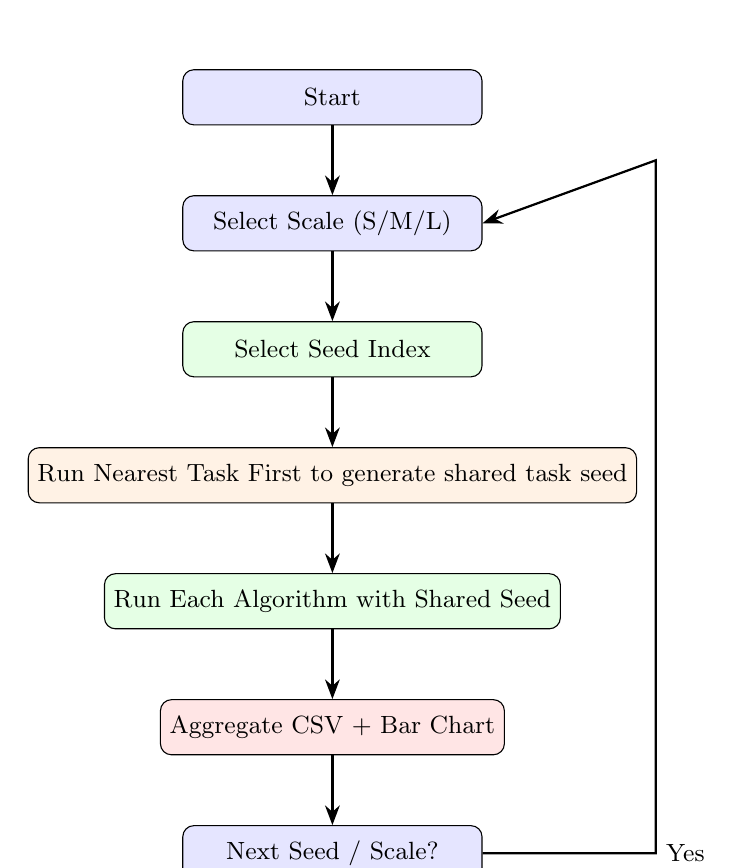
\begin{tikzpicture}[
        node distance=1.6cm,
        proc/.style={rectangle, draw, rounded corners, minimum width=3.8cm, minimum height=0.7cm, align=center, font=\small},
        arrow/.style={-{Stealth[length=2.5mm]}, thick},
    ]

        \node[proc, fill=blue!10] (start) {Start};
        \node[proc, fill=blue!10, below of=start] (scale) {Select Scale (S/M/L)};
        \node[proc, fill=green!10, below of=scale] (seed) {Select Seed Index};
        \node[proc, fill=orange!10, below of=seed] (gen) {Run Nearest Task First to generate shared task seed};
        \node[proc, fill=green!10, below of=gen] (loop) {Run Each Algorithm with Shared Seed};
        \node[proc, fill=red!10, below of=loop] (csv) {Aggregate CSV + Bar Chart};
        \node[proc, fill=blue!10, below of=csv] (next) {Next Seed / Scale?};

        \draw[arrow] (start) -- (scale);
        \draw[arrow] (scale) -- (seed);
        \draw[arrow] (seed) -- (gen);
        \draw[arrow] (gen) -- (loop);
        \draw[arrow] (loop) -- (csv);
        \draw[arrow] (csv) -- (next);
        \draw[arrow] (next.east) -- ++(2.2,0) node[right,font=\small] {Yes} -- ++(0,8.8) -- (scale.east);

    \end{tikzpicture}
    \caption{Shared-Seed Experimental Flow}
    \label{fig:exp-flow}
\end{figure}

Key design decisions:
\begin{itemize}[leftmargin=4em]
    \item \textbf{Seed generation:} For each (scale, seed) pair, Nearest Task First runs first without a preset seed. The resulting task sequence is saved for reuse.
    \item \textbf{Fair comparison:} All ten algorithms replay the \emph{identical} task sequence by loading the same seed file; only the scheduling strategy differs.
    \item \textbf{Seed counts:} Small scale uses 2 seeds; medium and large scales use 1 seed each, yielding 4 independent task sequences across all scales.
    \item \textbf{Total runs:} $4 \text{ seeds} \times 10 \text{ algorithms} = 40$ headless simulation runs.
    \item \textbf{Configuration isolation:} Each run writes its own configuration and log under a dedicated experiment output directory.
\end{itemize}

\subsection{Benchmark Runner Implementation}

The benchmark runner automates the following steps:

\begin{enumerate}[leftmargin=4em]
    \item Load base YAML configs for small, medium, and large scales.
    \item For each seed: generate (or reuse) the shared task seed via Nearest Task First.
    \item Iterate all ten algorithms, changing only the strategy and the seed file reference.
    \item Invoke the headless backend for each run.
    \item Parse the results block from each experiment log.
    \item Write per-seed CSV summaries and comparison bar charts.
\end{enumerate}

This pipeline ensures reproducibility: re-running the benchmark can skip already-completed runs and resume from incomplete seeds.

\section{Evaluation Metrics System}

Each simulation run records the following metrics (all time-based values in simulation seconds unless noted):

\begin{table}[H]
    \centering
    \caption{Evaluation Metrics System}
    \label{tab:metrics}
    \reporttableset{0.98\textwidth}
    \begin{reporttabular}{>{\raggedright\arraybackslash}l c >{\raggedright\arraybackslash}l}
        \toprule
        \textbf{Metric} & \textbf{Calculation} & \textbf{Interpretation} \\
        \midrule
        Completion Rate & $\dfrac{N_{\text{completed}}}{N_{\text{total}}}$ & Task processing capability \\
        On-time Rate    & $\dfrac{N_{\text{on-time}}}{N_{\text{completed}}}$ & Timeliness \\
        Total Score     & $\sum \text{score}(T_i)$ & Overall reward \\
        Avg Completion Time & $\dfrac{1}{N}\sum(t_{\text{finish}} - t_{\text{create}})$ & Response speed (sim.\,s) \\
        Throughput      & $\dfrac{N_{\text{completed}}}{\text{sim.\ hours}}$ & System efficiency \\
        Total Distance  & $\sum_v \text{dist}(v)$ & Energy cost \\
        Distance StdDev & $\sigma(\{\text{dist}(v)\})$ & Load balance \\
        Simulation Duration & --- & Total simulation time consumed \\
        Wall Duration   & --- & Real-world runtime (reference only) \\
        Stranded Vehicles & --- & Safety / robustness indicator \\
        \bottomrule
    \end{reporttabular}
\end{table}

\subsection{Algorithm Selection Criteria}

When comparing algorithms, we use a multi-criteria decision approach:

\begin{itemize}[leftmargin=4em]
    \item \textbf{Primary criterion:} Total Score --- directly reflects the final payoff of the strategy under the unified scoring formula.
    \item \textbf{Secondary criteria:} Completion Rate and On-time Rate --- reflect service quality.
    \item \textbf{Auxiliary criteria:} Avg Completion Time and Throughput --- reflect efficiency in simulation time.
    \item \textbf{Reference criteria:} Total Distance, Distance StdDev, and Stranded Vehicles --- reflect resource utilization and robustness.
    \item \textbf{Runtime reference:} Wall-clock duration is logged but not used for ranking, since all algorithms share the same simulation-time model.
\end{itemize}

Per-seed results are aggregated into CSV files and visualized as grouped bar charts (Total Score and Completion Rate) for direct cross-algorithm comparison within each scale.

% ============================================
% Chapter 5: Results and Analysis
% ============================================

\chapter{Results and Analysis}

This chapter presents the dynamic scheduling benchmark results from \texttt{experiments/dynamic\_benchmark/}. All algorithms under the same scale share an identical task-generation seed; small scale is averaged over two seeds, while medium and large scales use one seed each. All time-based metrics are in simulation seconds.

\section{Small-Scale Results}

\subsection{Performance Table}

The small-scale configuration uses 3 vehicles, 1 charging station, and a task budget of 20. Table~\ref{tab:small-results} reports the mean over seed~1 and seed~2 (11--12 tasks settled per run).

\begin{table}[H]
    \centering
    \caption{Small-Scale Dynamic Benchmark Results (mean of 2 seeds)}
    \label{tab:small-results}
    \reporttableset{0.98\textwidth}
    \begin{reporttabular}{>{\raggedright\arraybackslash}l cccc}
        \toprule
        \textbf{Algorithm} & \textbf{Comp.(\%)} & \textbf{On-time(\%)} & \textbf{Total Score} & \textbf{Avg Time (s)} \\
        \midrule
        RL Batch                 & 100.0 & 73.3 & $\mathbf{1262.4}$ & 5974 \\
        SA Score Search          & 100.0 & 72.5 & 1243.9 & 4190 \\
        DFS Score Search         & 100.0 & \textbf{81.7} & 1242.4 & 4888 \\
        Nearest Task First       & 100.0 & 68.3 & 1238.4 & 5177 \\
        Regional Planning        & 100.0 & 72.5 & 1171.0 & 5304 \\
        Priority First           & 100.0 & 72.5 & 1166.4 & 4564 \\
        Heaviest Task First      & 100.0 & 63.3 & 1066.1 & 5531 \\
        Cluster Auction MAS      & 100.0 & 64.2 & 1037.4 & 5155 \\
        Relay Handoff            & 100.0 & 64.2 & 1030.6 & 5793 \\
        Earliest Deadline First  & 100.0 & 72.5 & 940.7 & 4717 \\
        \bottomrule
    \end{reporttabular}
\end{table}

\begin{figure}[H]
    \centering
    \includegraphics[width=0.92\textwidth]{chapters/comparison0.png}
    \caption{Small-scale total score comparison seed~1.}
    \label{fig:small-score}
\end{figure}



\begin{figure}[H]
    \centering
    \includegraphics[width=0.92\textwidth]{chapters/comparison00.png}
    \caption{Small-scale total score comparison seed~2.}
    \label{fig:small-score}
\end{figure}




\subsection{Analysis}

\begin{itemize}[leftmargin=4em]
    \item All ten algorithms achieve \textbf{100\% completion} on both seeds; differentiation comes from total score and on-time rate.
    \item Search-based batch loaders (\textbf{RL Batch}, \textbf{SA Score Search}, \textbf{DFS Score Search}) occupy the top tier (1242--1262 mean score). \textbf{DFS Score Search} also yields the highest mean on-time rate (81.7\%).
    \item \textbf{Earliest Deadline First} scores lowest (940.7 mean), indicating that deadline-only sorting is insufficient when batch loading and battery constraints dominate.
    \item Seed~2 is more volatile: \textbf{Earliest Deadline First} drops to 699.1 while \textbf{DFS Score Search} reaches 1142.6 with 83.3\% on-time, confirming sensitivity to task sequence even under shared infrastructure.
    \item Cooperative strategies (\textbf{Relay Handoff}, \textbf{Cluster Auction MAS}) do not outperform greedy baselines at this scale, likely because the fleet is small and handoff overhead is not yet justified.
\end{itemize}

\section{Medium-Scale Results}

\subsection{Performance Table}

The medium-scale run uses 6 vehicles, 2 charging stations, and settles 49 tasks. Results from seed~1 are shown in Table~\ref{tab:medium-results}.

\begin{table}[H]
    \centering
    \caption{Medium-Scale Dynamic Benchmark Results (seed~1, 49 tasks)}
    \label{tab:medium-results}
    \reporttableset{0.98\textwidth}
    \begin{reporttabular}{>{\raggedright\arraybackslash}l cccc}
        \toprule
        \textbf{Algorithm} & \textbf{Comp.(\%)} & \textbf{On-time(\%)} & \textbf{Total Score} & \textbf{Avg Time (s)} \\
        \midrule
        DFS Score Search         & 100.0 & 53.1 & $\mathbf{3824.3}$ & 6990 \\
        RL Batch                 & 100.0 & 53.1 & 3795.3 & 6311 \\
        SA Score Search          & 100.0 & 51.0 & 3716.2 & 7353 \\
        Nearest Task First       & 100.0 & \textbf{57.1} & 3377.2 & 7118 \\
        Relay Handoff            & 100.0 & 51.0 & 2913.1 & 7503 \\
        Priority First           & 100.0 & 40.8 & 2824.1 & 8869 \\
        Regional Planning        & 100.0 & 49.0 & 2385.3 & 7099 \\
        Cluster Auction MAS      & 100.0 & 49.0 & 2385.3 & 7145 \\
        Heaviest Task First      & 100.0 & 40.8 & 2112.6 & 9240 \\
        Earliest Deadline First  & 100.0 & 46.9 & 1716.3 & 8190 \\
        \bottomrule
    \end{reporttabular}
\end{table}

\begin{figure}[H]
    \centering
    \includegraphics[width=0.92\textwidth]{chapters/comparison1.png}
    \caption{Medium-scale total score comparison (seed~1, 49 tasks).}
    \label{fig:medium-score}
\end{figure}

\subsection{Analysis}

\begin{itemize}[leftmargin=4em]
    \item Completion remains \textbf{100\%} for all algorithms, but on-time rates fall to 41--57\%, reflecting tighter deadlines relative to fleet capacity.
    \item \textbf{DFS Score Search} (3824.3) and \textbf{RL Batch} (3795.3) clearly outperform greedy baselines, validating explicit batch-score optimization under higher load.
    \item Simple greedy rules diverge: \textbf{Nearest Task First} stays competitive (3377.2) while \textbf{Earliest Deadline First} collapses to 1716.3 --- deadline sorting alone cannot compensate for poor batch composition.
    \item Multi-vehicle coordinators (\textbf{Regional Planning}, \textbf{Cluster Auction MAS}) score 2385.3 with identical outcomes on this seed, suggesting similar package-decomposition behavior but no advantage over search-based per-vehicle batching here.
    \item The score gap between best and worst widens to 2108 points (3824.3 vs.\ 1716.3), showing that algorithm choice matters substantially at medium scale.
\end{itemize}

\section{Large-Scale Results}

\subsection{Performance Table}

The large-scale run uses 12 vehicles, 4 charging stations, and settles 32 tasks within the generation window. Table~\ref{tab:large-results} lists seed~1 results.

\begin{table}[H]
    \centering
    \caption{Large-Scale Dynamic Benchmark Results (seed~1, 32 tasks)}
    \label{tab:large-results}
    \reporttableset{0.98\textwidth}
    \begin{reporttabular}{>{\raggedright\arraybackslash}l cccc}
        \toprule
        \textbf{Algorithm} & \textbf{Comp.(\%)} & \textbf{On-time(\%)} & \textbf{Total Score} & \textbf{Avg Time (s)} \\
        \midrule
        Cluster Auction MAS      & 96.9 & 96.8 & $\mathbf{3278.7}$ & 1194 \\
        SA Score Search          & 100.0 & \textbf{96.9} & 3221.3 & 1089 \\
        Regional Planning        & 100.0 & 96.9 & 3045.0 & 1530 \\
        Heaviest Task First      & 100.0 & 93.8 & 2982.8 & 1395 \\
        RL Batch                 & 100.0 & 93.8 & 2907.9 & 1305 \\
        Earliest Deadline First  & 100.0 & 93.8 & 2907.9 & 1323 \\
        DFS Score Search         & 100.0 & 93.8 & 2907.9 & 1305 \\
        Priority First           & 100.0 & 93.8 & 2727.1 & 1377 \\
        Nearest Task First       & 100.0 & 96.9 & 2652.6 & 1368 \\
        Relay Handoff            & 100.0 & 93.8 & 2244.0 & 1764 \\
        \bottomrule
    \end{reporttabular}
\end{table}

\begin{figure}[H]
    \centering
    \includegraphics[width=0.92\textwidth]{chapters/comparison2.png}
    \caption{Large-scale total score comparison (seed~1, 32 tasks).}
    \label{fig:large-score}
\end{figure}

\subsection{Analysis}

\begin{itemize}[leftmargin=4em]
    \item Most algorithms complete all 32 tasks; \textbf{Cluster Auction MAS} stops at 31/32 (96.9\% completion) with one timeout, yet still achieves the highest total score (3278.7) on this seed.
    \item \textbf{SA Score Search} balances score (3221.3) with full completion and the joint-best on-time rate (96.9\%).
    \item \textbf{Relay Handoff} scores lowest (2244.0) despite 100\% completion --- relay negotiation adds route overhead without sufficient cargo-rebalancing benefit on this instance.
    \item Several batch-search variants (\textbf{RL Batch}, \textbf{DFS Score Search}, \textbf{Earliest Deadline First}) converge to identical scores (2907.9), indicating diminishing returns of search when the pending pool is small at each decision step.
    \item Compared with medium scale, absolute scores drop because fewer tasks are settled before the generation cutoff, highlighting that scale configuration affects both difficulty and score magnitude.
\end{itemize}

\section{Comparison with Static Gurobi Solver}


\begin{figure}[H]
    \centering
    \includegraphics[width=0.92\textwidth]{chapters/gurobi.png}
    \caption{static result for gurobi.}
    \label{fig:small-score}
\end{figure}



As an supplementary baseline, we also ran the static omniscient solver (Gurobi) on the same task-generation seeds. Table~\ref{tab:static-gurobi} summarizes those results.

\begin{table}[H]
    \centering
    \caption{Static Omniscient Solver Results (Gurobi)}
    \label{tab:static-gurobi}
    \begin{reporttabular}{lccc}
        \toprule
        \textbf{Scale} & \textbf{Total Score} & \textbf{Completed / Total} & \textbf{Completion Rate} \\
        \midrule
        Small  & 877.9  & 10 / 10 & 100.0\% \\
        Medium & 3003.6 & 20 / 20 & 100.0\% \\
        Large  & 4407.0 & 38 / 39 & 97.4\%  \\
        \bottomrule
    \end{reporttabular}
\end{table}

The static solver results differ substantially from the dynamic benchmark and do not consistently dominate:
\begin{itemize}[leftmargin=4em]
    \item At \textbf{small} and \textbf{medium} scales, the best dynamic strategies (\textbf{RL Batch} at 1262.4; \textbf{DFS Score Search} at 3824.3) \emph{exceed} the static scores (877.9 and 3003.6 respectively).
    \item At \textbf{large} scale, the static total (4407.0) appears higher in absolute terms, but it covers a different settled task count (38/39 vs.\ 32/32 for most dynamic runs), so direct comparison is limited.
    \item We suspect the gap is partly caused by \textbf{time-penalty modeling} in the MIP formulation: overdue and timing-related penalty terms may push the solver toward conservative routes that score poorly under our unified dynamic scoring function, and in some cases yield solutions worse than online heuristics.
\end{itemize}

\section{Cross-Scale Summary}

Table~\ref{tab:cross-scale-best} highlights the best-performing dynamic strategy per scale.

\begin{table}[H]
    \centering
    \caption{Best Dynamic Strategy per Scale}
    \label{tab:cross-scale-best}
    \reporttableset{0.98\textwidth}
    \begin{reporttabular}{llcc>{\raggedright\arraybackslash}l}
        \toprule
        \textbf{Scale} & \textbf{Best Algorithm} & \textbf{Score} & \textbf{On-time} & \textbf{Notes} \\
        \midrule
        Small  & RL Batch            & 1262.4 & 73.3\% & Mean of 2 seeds; DFS best on-time (81.7\%) \\
        Medium & DFS Score Search    & 3824.3 & 53.1\% & Search-based batching clearly wins \\
        Large  & Cluster Auction MAS & 3278.7 & 96.8\% & One timeout; SA Score Search best balanced \\
        \bottomrule
    \end{reporttabular}
\end{table}






Key findings across all experiments:

\begin{itemize}[leftmargin=4em]
    \item \textbf{No single algorithm wins everywhere.} Search-based loaders excel at medium scale; auction-based coordination peaks at large scale; RL/SA variants are strong at small scale.
    \item \textbf{Completion vs.\ quality.} All dynamic runs achieve near-perfect completion; on-time rate and total score are the primary discriminators, especially at medium scale where on-time drops below 60\%.
    \item \textbf{Greedy baselines remain useful.} \textbf{Nearest Task First} stays in the upper tier at small and medium scales with minimal implementation cost.
    \item \textbf{Cooperative strategies are scale-dependent.} \textbf{Relay Handoff} underperforms at all scales tested; \textbf{Cluster Auction MAS} becomes competitive only when the fleet and task pool are large enough.
    \item \textbf{Static vs.\ dynamic.} Gurobi static planning does not reliably beat online dynamic policies under the same scoring rules, suggesting that model fidelity (especially time penalties) matters as much as optimality guarantees.
\end{itemize}

% ============================================
% Chapter 6: Conclusion and Reflections
% ============================================

\chapter{Conclusion and Reflections}

\section{Project Summary}

This project designed and implemented NEFT, a simulation platform for electric logistics fleet cooperative dispatching, and evaluated ten dynamic scheduling strategies under controlled, reproducible conditions. The main outcomes are:

\subsection{Simulation System}

\begin{itemize}[leftmargin=4em]
    \item Built a graph-based road network (OpenStreetMap / OSMnx) with Dijkstra shortest-path routing and a simulation-time clock decoupled from wall-clock execution.
    \item Modeled three vehicle types, dynamic task generation with shared seeds, charging-station queuing, and a unified scoring function used for both settlement and batch-selection objectives.
    \item Delivered a snapshot-to-command scheduling interface with shared utility modules, enabling fair comparison and rapid prototyping of new strategies.
    \item Implemented a FastAPI + WebSocket + AMap visualization front-end for real-time monitoring.
\end{itemize}

\subsection{Algorithm Portfolio}

\begin{itemize}[leftmargin=4em]
    \item \textbf{Greedy baselines (4):} Nearest Task First, Heaviest Task First, Earliest Deadline First, Priority First.
    \item \textbf{Search-based batch loaders (3):} DFS Score Search, SA Score Search, RL Batch.
    \item \textbf{Multi-vehicle coordination (3):} Regional Planning, Cluster Auction MAS, Relay Handoff.
    \item All strategies share battery pre-check, mid-route recharge simulation, and charging-station load balancing through common decision templates.
\end{itemize}

\subsection{Experimental Findings}

\begin{itemize}[leftmargin=4em]
    \item Ran 40 headless dynamic benchmarks (4 shared seeds $\times$ 10 algorithms) under identical task sequences per seed.
    \item Dynamic algorithms achieve near-perfect completion; total score and on-time rate separate strategies, especially at medium scale (on-time 41--57\%).
    \item \textbf{DFS Score Search} and \textbf{RL Batch} lead at medium scale ($\approx$3800 points); \textbf{RL Batch} and search variants lead at small scale; \textbf{Cluster Auction MAS} scores highest at large scale on the tested seed.
    \item A supplementary Gurobi static solver baseline did not consistently outperform dynamic policies; at small and medium scales several dynamic strategies scored higher, possibly because time-penalty terms in the MIP model distort the objective relative to the online scoring function.
\end{itemize}

\section{Lessons Learned}

\begin{enumerate}[leftmargin=4em]
    \item \textbf{Fair comparison requires infrastructure, not just algorithms.} The snapshot interface and shared task seeds were essential; without them, score differences would reflect random task noise rather than strategy quality.
    \item \textbf{Batch loading dominates medium-scale performance.} When pending queues grow, explicit search over feasible batches (DFS / RL) substantially beats single-key greedy sorting.
    \item \textbf{Cooperation has a scale threshold.} Relay and auction mechanisms need sufficient fleet size and geographic task spread; otherwise coordination overhead hurts more than it helps.
    \item \textbf{Static optima $\neq$ dynamic benchmark winners.} Exact solvers are only meaningful when the mathematical model faithfully encodes the same penalties and timing semantics as the simulator; mismatched time-penalty modeling can make ``optimal'' static plans score worse than simple online heuristics.
    \item \textbf{Visualization accelerates debugging.} Map-based route display exposed charging and routing edge cases that log inspection alone would have missed.
\end{enumerate}

\section{Future Work}

\begin{itemize}[leftmargin=4em]
    \item Refine the static MIP formulation so that deadline and overdue penalties align exactly with the dynamic scoring module, enabling a fair static-vs-dynamic gap analysis.
    \item Extend benchmarks with more seeds per scale and report mean $\pm$ std.\ dev.\ for statistical confidence.
    \item Tune cooperative strategies (relay thresholds, auction bid weights) and test on denser task streams where handoff should pay off.
    \item Explore hybrid policies that switch between greedy, search, and multi-agent modes based on pending-queue size and fleet utilization.
\end{itemize}

\section{Team Reflections}

This project took us from textbook scheduling concepts to a working system where vehicles move on a real map, charge at stations, and compete under a unified score. Implementing ten strategies on one interface showed how much engineering effort lies beyond the core algorithm --- battery safety, seed reproducibility, and simulation-time semantics all shaped the final rankings as much as the dispatching logic itself.

The experimental phase changed how we evaluate algorithms: a single impressive run is misleading, but shared seeds across ten strategies revealed clear patterns --- search wins at medium load, coordination matters at large scale, and simple nearest-neighbor rules remain a strong baseline. Working in a team mirrored real software practice: simulation core, algorithms, visualization, and analysis had to integrate through clear contracts, much like the snapshot-to-command design we built for the schedulers themselves.


\end{document}